
\subsubsection{Partitore resistivo}
%
    Schema del ciruito:
    %
    \begin{figure}[H]
    \centering
    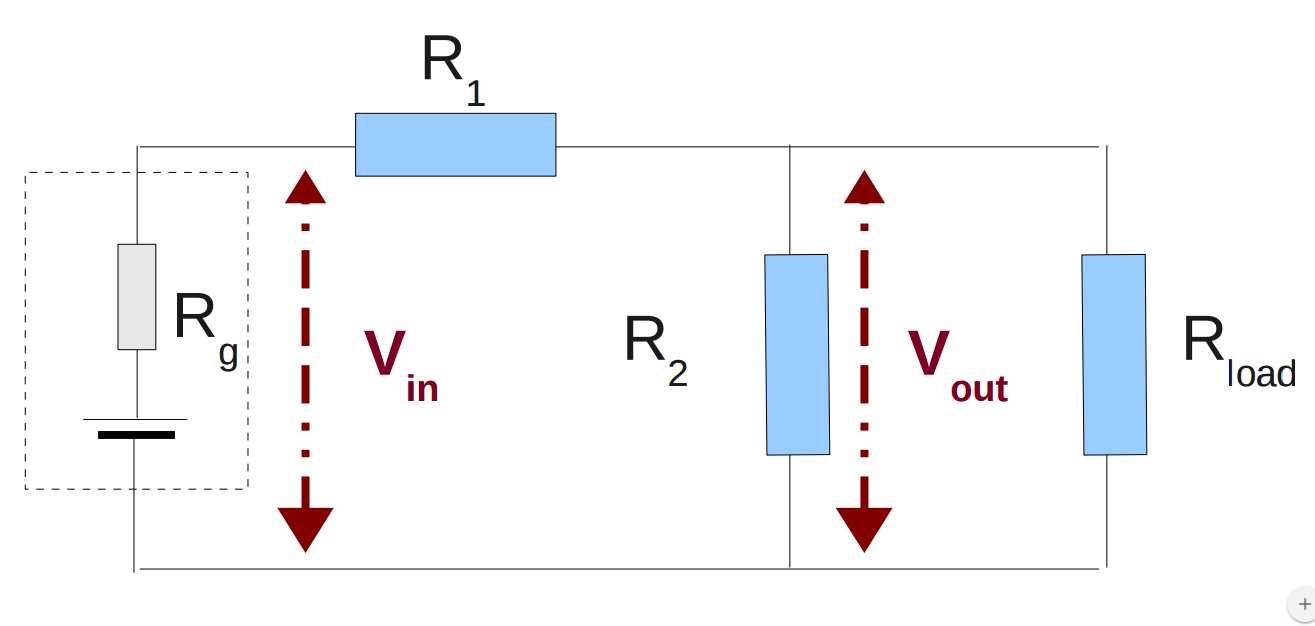
\includegraphics[scale=.25]{Grafici/C1_P2.png}
    \end{figure} 

    Affinchè $V_{out}$ sia circa metà di $V_{in}$ senza $R_L$, si ha che $R_1$ e $R_2$ devono essere circa uguali, in modo che la caduta di potenziale sia distribuita sui due resistori in modo uguale.\\
    Lasciando $R_1$ e $R_2$ uguali, abbiamo verificato due casi: resistenze basse e alte.\\
    Affinchè la caduta di potenziale su $R_L$ sia circa indipendente dal suo valore, occorre che $R_2$ sia molto minore di $R_L$ affinchè abbia peso maggiore nella resistenza equivalente, come dimostrato nei seguenti calcoli:
    $$ \Delta V = V_{R_1} + V_{R_L} = I R_1 + I \frac{R_2 R_L}{R_2 + R_L} = I R_1 + \frac{I R_2}{1 + \frac{R_2}{R_L}}  $$
    Se $ R_2$ molto minore di $R_L$, il denominatore tende a 1 e dunque $V_{R_L}$ non dipende da $R_L$.\\\\
    %
    \textbf{Dati sperimentali}\\\\
    %
    \textbf{Resistenze basse}\\
    %
    $R_L$ (kOhm) =	0.266	$\pm$ 0.001\\
    $R_2$ kOhm) =	0.268   $\pm$ 0.001\\
    %
    %
    %
    \begin{table}[H]
\centering
\caption{Resistenze basse}
\begin{tabular}{|c|c|c|}
\hline
$R_L$	&	$V_{in}$ 	&	$V_{out}$	\\
$[kOhm]$	&	$[V]$	&	$[V]$	\\
$\pm 1 kOhm$ 	&	$\pm 0.01 V$	&	$\pm 0.001 V$	\\ \hline
100	&	1.50	&	0.754	\\
100	&	3.00	&	1.503	\\
100	&	5.00	&	2.501	\\ \hline
149	&	1.50	&	0.757	\\
149	&	3.00	&	1.504	\\
149	&	5.00	&	2.500	\\ \hline
981	&	1.50	&	0.756	\\
981	&	3.00	&	1.505	\\
981	&	5.00	&	2.504	\\ \hline
\end{tabular}
\label{}
\end{table}
    %
    %
    Il seguente grafico mostra tutti i dati sulla stessa canvas. 
    % grafico
    \begin{figure}[H]
    \centering
    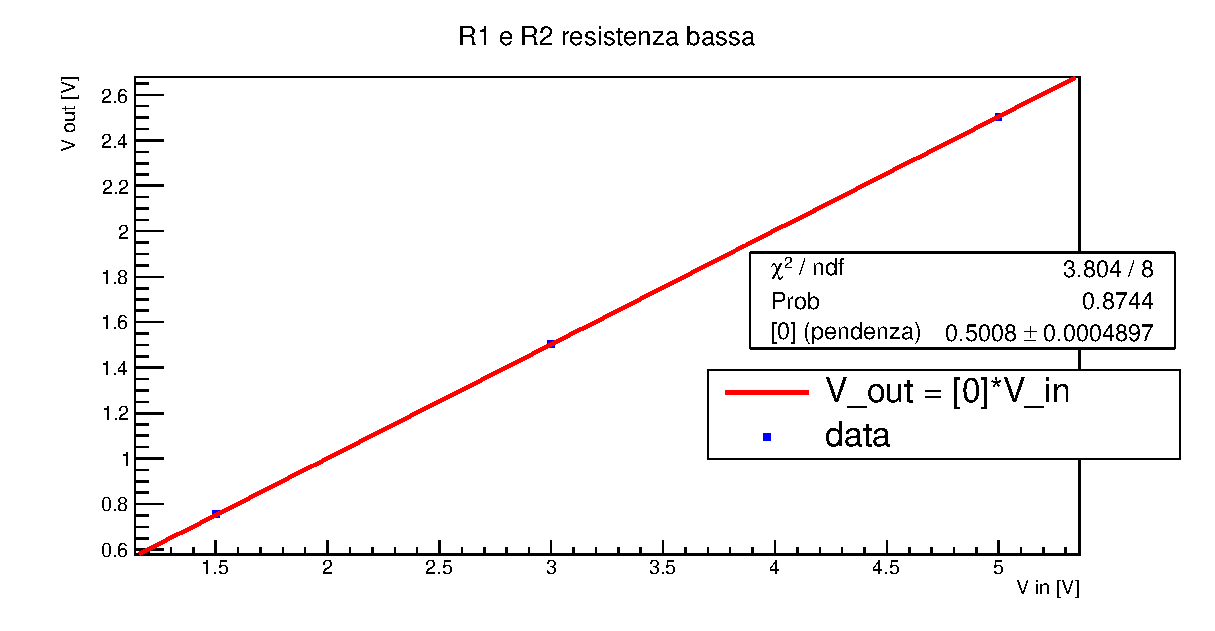
\includegraphics[scale=.7]{Grafici/C1_P2_partResLow.eps}
    \end{figure}
    %
    Si osserva che:
    \begin{itemize}
        \item  I valori sono 9 come riportato nella tabella, ma sono a tre a tre molto simili, quindi non si riescono a distinguere. Da questo segue che la caduta di tensione in $R_L$ non dipende da $R_L$. Infatti a parità di $V_{in}$, cambiando $R_L$ il $V_{out}$ non cambia.
        \item $V_{out} = 0.5 \cdot V_{in}$, con un chi quadro ridotto di 3.8/8.
    \end{itemize}
%
    \textbf{Resistenze alte}\\\\		
    $R_1$ (kOhm) =	978 $\pm$ 1\\
    $R_2$ (kOhm) =	981 $\pm$ 1\\
    %
    %
    \begin{table}[H]
\centering
\caption{Resistenze alte}
\begin{tabular}{|c|c|c|}
\hline
$R_L$	&	$V_{in}$ 	&	$V_{out}$	\\
$[kOhm]$	&	$[V]$	&	$[V]$	\\
$\pm 1 kOhm$ 	&	$\pm 0.01 V$	&	$\pm 0.001 V$	\\ \hline
0.677	&	5.24	&	0.004	\\
0.677	&	10.00	&	0.007	\\
0.677	&	14.00	&	0.010	\\ \hline
15.97	&	3.00	&	0.047	\\
15.97	&	5.00	&	0.079	\\
15.97	&	7.00	&	0.110	\\ \hline
100.1	&	3.00	&	0.253	\\
100.1	&	5.00	&	0.421	\\
100.1	&	7.00	&	0.589	\\ \hline
\end{tabular}
\label{}
\end{table}
    %
    I seguenti tre grafici mostrano i dati, suddivisi per $R_L$ utilizzata.
    %
    % grafico
    \begin{figure}[H]
    \centering
    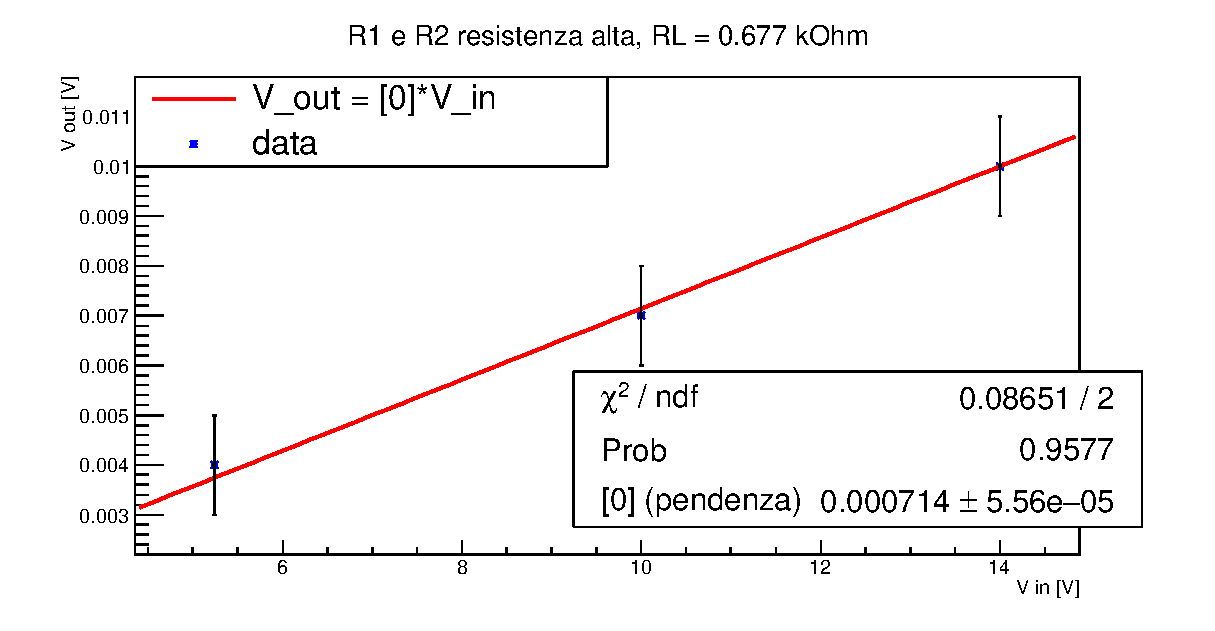
\includegraphics[scale=.7]{Grafici/C1_P2_partResHigh1.eps}
    \end{figure}
    
    \begin{figure}[H]
    \centering
    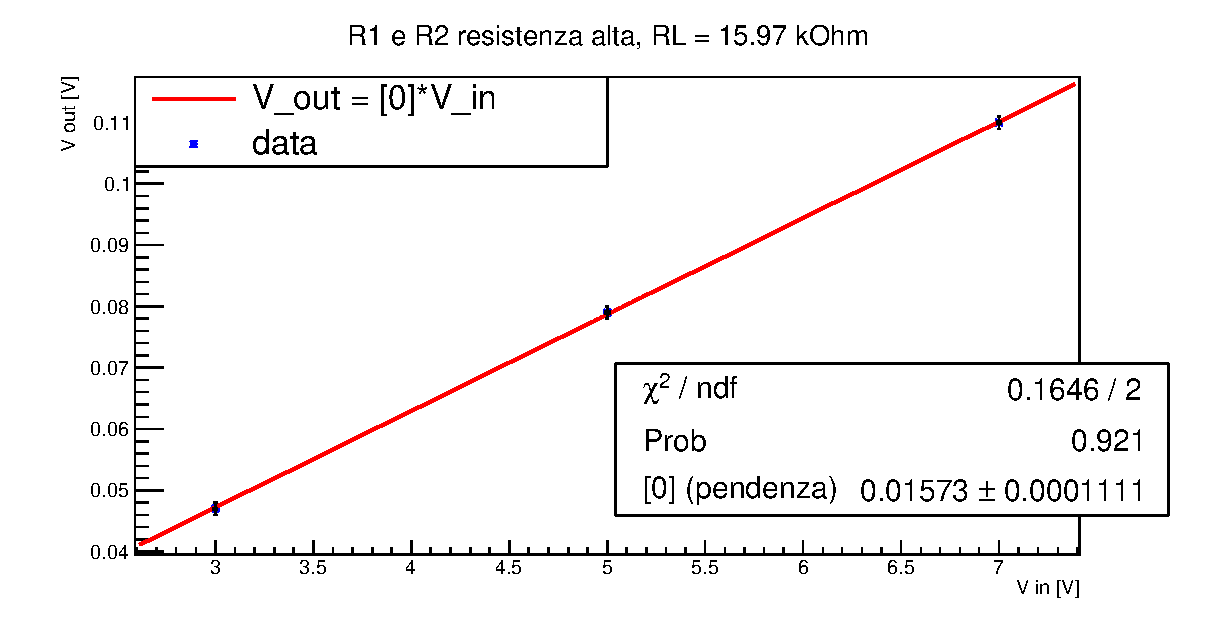
\includegraphics[scale=.7]{Grafici/C1_P2_partResHigh2.eps}
    \end{figure}
    
    \begin{figure}[H]
    \centering
    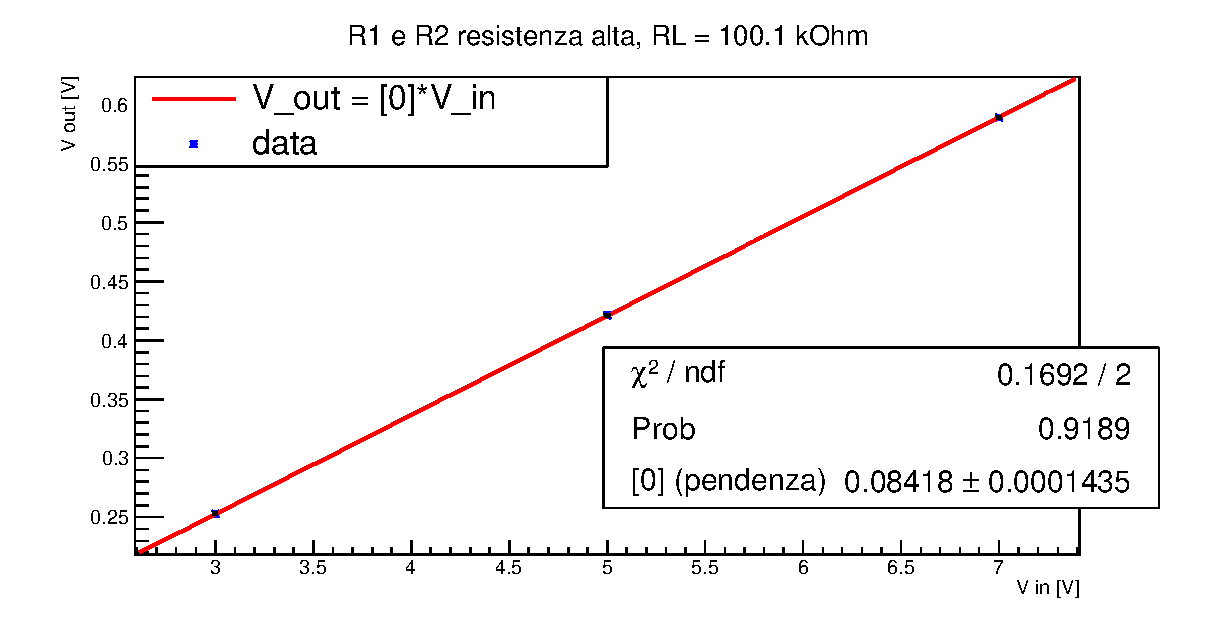
\includegraphics[scale=.7]{Grafici/C1_P2_partResHigh3.eps}
    \end{figure}
    %
    %
    Si è dunque verificato che:
    \begin{itemize}
        \item La caduta di tensione in $R_L$  dipende da $R_L$. Infatti a parità di $V_{in}$, cambiando $R_L$ il $V_{out}$ cambia.
        \item Non è vero che $V_{out} = 0.5 \cdot V_{in}$.
    \end{itemize}
%    
\subsubsection{Approfondimento: Potenza massima trasferibile}
    % Dati resistenze
    Si è tolta $R_2$ dal circuito.\\
    Per la misura di $R_g$ abbiamo utilizzato una resistenza $R_1$ da $10.1 \Omega$, e ricavato $R_g$ da
    $$Rg = \frac{fem-V}{I} = 1.4 \Omega $$
    %%manca errore Rg
    con $fem$ = forza elettromotrice erogata da generatore,
    $V$ = Differenza di potenziale misurata ai capi del resistore, $I$ = corrente che scorre attraverso il circuito.\\
    $R_g$ espresso come media delle misure e errore calcolato con le formule di propagazione.\\
%
    % tabella misura Rg
       \begin{table}[H]
    \centering
    \caption{Misura di $R_g$}
    \begin{tabular}{|c|c|c|c|}
    \hline
        $fem$ & Tensione (V) & Corrente (A) & Rg \\ \hline
        V & V & A & $\Omega$ \\ \hline
        $\pm$0.01 & $\pm$0.001 & $\pm$ 0.001 & 0.02 \\ \hline
        3.00 & 2.626 & 0.267 & 1.401 \\ 
        2.50 & 2.189 & 0.222 & 1.401 \\ 
        2.00 & 1.756 & 0.178 & 1.371 \\ 
        1.50 & 1.323 & 0.135 & 1.311 \\ \hline
    \end{tabular}
    \label{}
    \end{table}
%
    Per la misura della massima potenza dissipabile su $R_L$ abbiamo utilizzato una resistenza $R_1= 149 k\Omega$, nota $R_g = 0.0014 k\Omega$, e una $fem$ da $7.5 V$. \\
 %
    La previsione teorica del massimo di potenza dissipata in $R_L$ è ottenuta massimizzando la funzione
    $$P=I^2\cdot R_{L} = \frac{fem^2 R_L}{(R_g + R_1 + R_L)^2} $$
    dove la corrente è stata ricavata dall'equazione del circuto:   
    $$fem- IR_g = IR_1 + I R_L \Rightarrow I = fem / (R_g+R_1+R_L)$$
    ponendo $\frac{\partial P}{\partial R_L} = 0$, si trova:
    $$ R_L max = R_1+R_g = 149  k\Omega$$
%
    Le misure indicano un massimo di potenza in prossimità di $R_L = 150 k\Omega$.\\
    %
    Di seguito il grafico che mostra la curva della potenza dissipata in $R_L$, e una linea verticale che segna il massimo teorico, che si trova abbastanza vicino al massimo della curva. Abbiamo quindi verificato quanto dimostrato in teoria.\\   
    % Grafico RL / potenza
    \begin{figure}[H]
    \centering
    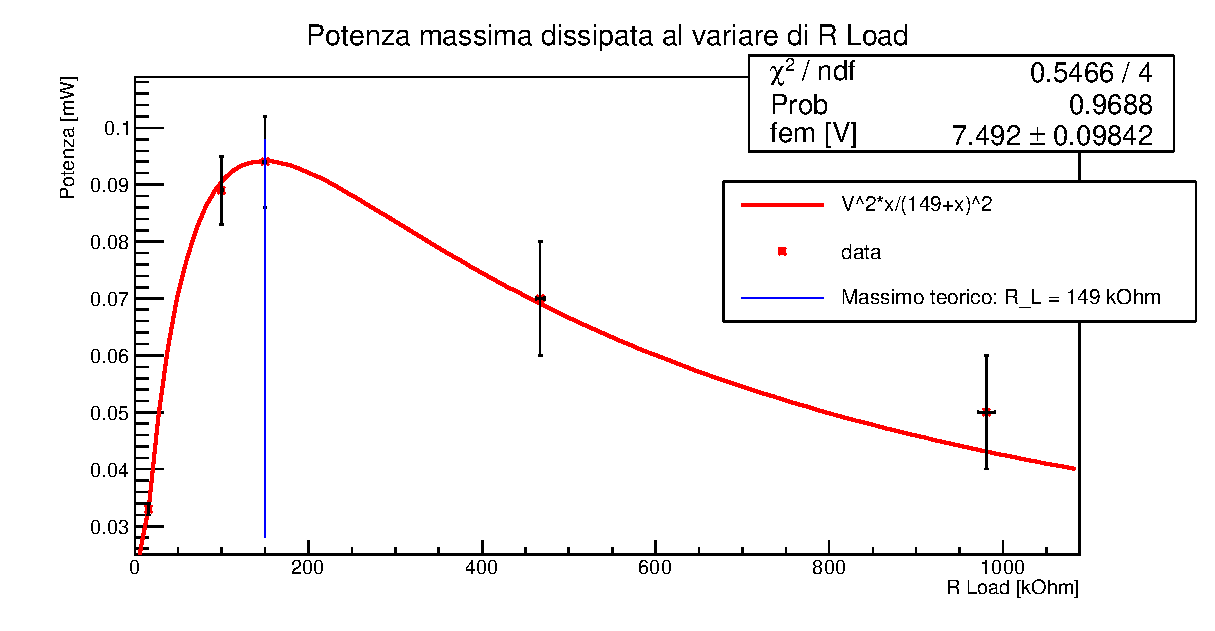
\includegraphics[scale=.7]{Grafici/C1_P2_maxPower.eps}
    \caption{Grafico Resistenza-Potenza trasferita}
    \label{fig:C1_P2_maxPower}
    \end{figure}
    

    
    
    
